\documentclass{article}
\usepackage[utf8]{inputenc}
\usepackage{hyperref}
\usepackage[letterpaper, portrait, margin=1in]{geometry}
\usepackage{enumitem}
\usepackage{amsmath}
\usepackage{amsthm}
\usepackage{booktabs}
\usepackage{graphicx}
\usepackage{float}
\usepackage{hyperref}
\usepackage[flushleft]{threeparttable}
\usepackage{textcomp}
\usepackage{amssymb}
\usepackage{dsfont}
\hypersetup{
colorlinks=true,
    linkcolor=black,
    filecolor=black,      
    urlcolor=blue,
    citecolor=black,
}
\usepackage{natbib}
\usepackage{yhmath}

\usepackage{titlesec}
\bibliographystyle{chicago}
\newcommand{\bib}{references.bib}
\newcommand\iid{\stackrel{\mathclap{iid}}{\sim}}
\newcommand\asym{\stackrel{\mathclap{a}}{\sim}}
\newcommand\convprob{\xrightarrow{p}}
\newcommand\convdist{\xrightarrow{d}}
\newcommand{\N}{\mathbb{N}}
\newcommand{\Z}{\mathbb{Z}}
\newcommand{\E}{\text{E}}
\newcommand{\V}{\text{Var}}
\newcommand{\Av}{\text{Avar}}
\newcommand{\se}{\text{se}}
\newcommand{\corr}{\text{Corr}}
\newcommand{\cov}{\text{Cov}}
\newcommand{\norm}{\text{Normal}}
\newcommand{\indep}{\perp \!\!\! \perp}

\begin{document}
% The tex content below is similar to the given main.tex
 
\title{Homework 4}
\author{Environmental Economics II\\
Maghfira Ramadhani}
\date{\today}
\maketitle

\section*{Problem 1 Python}
\begin{enumerate}
\item Figure \ref{f1:paralleltrend} shows that there's a parallel trend before the treatment started in Jan 2018. This is important to ensure that the treatment and control group are comparable before the treatment started.
\begin{figure}[H]
\centering
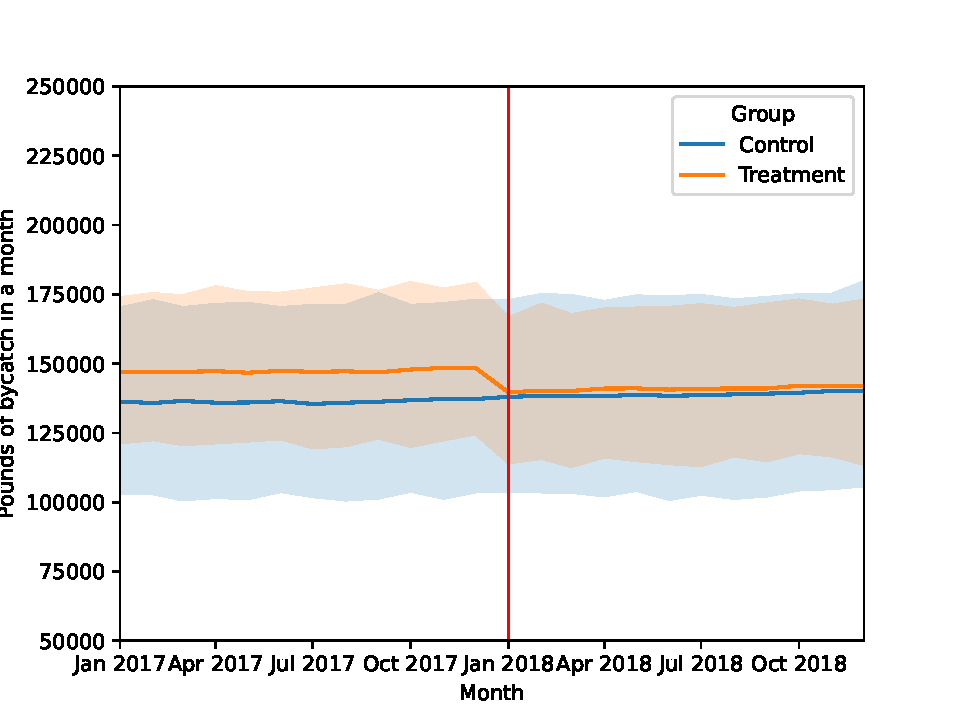
\includegraphics[scale = 0.7]{./figure/paralleltrend.pdf}
\caption{Bycatch by month plot}
\label{f1:paralleltrend}
\end{figure}

\item DID estimates by using sample analog
\begin{table}[H]\centering
\begin{threeparttable}
\caption{Parameter and average marginal effect estimates from Stata}
\label{t1:didstimates}
\begin{tabular}{rl}
\toprule
 & Sample analog value \\
\midrule
$\E[Y_{igt}|g(i)=treatment,t=Pre]=$ & 148430.64 \\
$\E[Y_{igt}|g(i)=treatment,t=Post]=$ & 139612.51 \\
$\E[Y_{igt}|g(i)=control,t=Pre]=$ & 137228.60 \\
$\E[Y_{igt}|g(i)=control,t=Post]=$ & 139612.51 \\
\midrule DID= & -9591.35 \\
\bottomrule
\end{tabular}

\end{threeparttable}
\end{table}

\item Estimating DID using different specification in Python
\begin{table}[H]\centering
    \begin{threeparttable}
    \caption{DID estimates from different specification}
    \label{t2:didstimatesspecification}
    \begin{tabular}{rccc}
\toprule
 & (a) & (b) & (c) \\
\midrule
DID estimates & -9591.35 & -8956.78 & -8436.28 \\
  & (3198.64) & (3135.04) & (2795.47) \\
\midrule Group FE & \checkmark & \checkmark & \checkmark \\
Month Indicator & \checkmark & \checkmark & \checkmark \\
Controls & $\times$ & $\times$ & \checkmark \\
Sample & Dec 2017 - Jan 2018 & Jan 2017 - Dec 2018 & Jan 2017 - Dec 2018 \\
\bottomrule
\end{tabular}

    \begin{tablenotes}
        \small \item Standard errors are clustered at firm. I used pyfixest package for the estimation, the documentation is available at \url{https://github.com/s3alfisc/pyfixest}.
    \end{tablenotes}
    \end{threeparttable}
\end{table}
\begin{enumerate}
    \item The following specification is used. 
    \begin{align}
        bycatch_{it} &= \alpha + \lambda_{t=2017}+ \gamma g(i) + \delta treat_{i,t} + \epsilon_{i,t} \label{e:spec1a}
    \end{align}
    By using sample from December 2017 and January 2018, the DID estimates is -9591.35 with a standard error of 3198.64. This means after the treatment started, the treated firms' bycatch yield is on average 9591.35 lbs less compared to the control group.
    \item The following specification is used. 
    \begin{align}
        bycatch_{it} &= \alpha + \lambda_{t}+ \gamma g(i) + \delta treat_{i,t} + \epsilon_{i,t} \label{e:spec1b}
    \end{align}
    By using sample from January 2017 and December 2018, the DID estimates is -8956.78 with a standard error of 3135.04. This means after the treatment started, the treated firms' bycatch yield is on average 8956.78 lbs less compared to the control group. Using this spefication we are now comparing the average of the entire after treatment period with the average of the entire before treatment period average, instead of only using 1 month of observations. This specification is more robust in capturing common time trends or seasonality of bycatch yields between both treated and untreated firms.

    \item The following specification is used. 
    \begin{align}
        bycatch_{it} &= \alpha + \lambda_{t}+ \gamma g(i) + \delta treat_{i,t} + \beta X_{i,t} + \epsilon_{i,t} \label{e:spec1b}
    \end{align}
    By using sample from January 2017 and December 2018, the DID estimates is -8436.28 with a standard error of 2795.47. In this specification, we include firm size, salmon yields, and shrimp yields as control variables. This specification is more robust in capturing common time trends or seasonality of bycatch yields between both treated and untreated firms, and also controlling for other factors that might affect bycatch yields.

    \item Table \ref{t2:didstimatesspecification} show the DID estimates from the different specification shown in part (a), (b), and (c). The estimates from part (a) is similar with the result from computing the sample analog in question 2. The estimates from part (b) is more precise than (a) due to the larger sample size. The estimates from part (c) is more precise than (b) due to the inclusion of control variables.
    
\end{enumerate}
\end{enumerate} 

\section*{Problem 2 Stata}
\begin{enumerate}
\item Estimating DID using different specification in Stata
\begin{table}[H]\centering
    \begin{threeparttable}
    \caption{DID estimates from different methods in Stata}
    \label{t3:stata_estimates}
    \begin{tabular}{l*{2}{c}}
\hline\hline
                    &\multicolumn{1}{c}{Parameter Estimates}&\multicolumn{1}{c}{AME Estimates}\\
\hline
Constant            &      -0.769&            \\
                    &[-1.848,0.310]&            \\
=1 if home received retrofit&       0.904&    -110.729\\
                    &[0.893,0.916]&[-130.589,-90.869]\\
Square feet of home &       0.894&       0.622\\
                    &[0.880,0.909]&[0.607,0.638]\\
Outdoor average temperature (\textdegree F)&       0.281&       2.851\\
                    &[0.039,0.524]&[-2.057,7.758]\\
\hline
Observations        &       1,000&       1,000\\
\hline\hline
\end{tabular}

    \begin{tablenotes}
        \small \item Standard errors are clustered at firm.
    \end{tablenotes}
    \end{threeparttable}
\end{table}
\begin{enumerate}
    \item The following specification is used.
    \begin{align}
        bycatch_{it} &= \alpha_i + \lambda_{t}+ \gamma g(i) + \delta treat_{i,t} + \beta X_{i,t} + \epsilon_{i,t} \label{e:spec2a}
    \end{align}
    The estimates is shown in Table \ref{t3:stata_estimates} column (a).
    \item Let $\tilde{y}_{it}=y_{it}-\bar{y}_i$ denote the time-demeaned variable. The following specification which is equivalent with equation \eqref{e:spec2a} is used.
    \begin{align}
        \widetilde{bycatch}_{it} &= \delta \widetilde{treat}_{i,t} + \beta \tilde{X}_{i,t} + \tilde{\epsilon}_{i,t} \label{e:spec2b}
    \end{align}
    Note that due to the time demeaning, firmsize which is time-invariant control variable is dropped from the regression. The estimates is shown in Table \ref{t3:stata_estimates} column (b).
    \item Comparing estimates from (b) to (a), it looks like the estimates from (b) is more precise than (a) due to the smaller standard errors. However, the time demeaning removes the time-invariant control variables, i.e. firm size, from the regression, which could be a problem if we are to identify the coefficient for those variable.
\end{enumerate}
\end{enumerate}
    
\end{document}